
\section{The Electric Field and the Electric Potential I}

\makelabheader %(Space for student name, etc., defined in master.tex)

\textbf{Objective}

\begin{itemize}
\item To investigate the electric field and potential of a point charge.
\end{itemize}

\textbf{Apparatus}

\begin{itemize}
\item Electric field and potential simulation entitled {\it EMField}.
\end{itemize}

\textbf{Introduction}

The direction of an electric field is the direction of the force on
a tiny positive test charge placed in the region of space where the
field is to be measured. If the magnitude of this test charge is infinitesimally
small, so small that it will not displace or disturb the charges that
are the source of the field, we can use the test charge to determine
quantitatively the strength of the electric field. The strength of
the electric field is taken to be the electric force, $F$, on the test
charge divided by the magnitude of the test charge, \( q_{t} \):
\( E=\frac{F}{q_{t}} \). The force (Coulomb's Law) between two charges,
\( q_{1} \) and \( q_{2} \), is \( F=k\frac{q_{1}q_{2}}{r^{2}} \),
where \( k \)= 9 x 10\( ^{9} \) Nm\( ^{2} \)/C\( ^{2} \). The units
of \( E \) are newtons per coulomb, so another way of describing the field
strength is to say it is the force experienced by a unit positive
test charge.

Recall from a previous laboratory exercise that the potential difference
between two points A and B, V\( _{B} \) - V\( _{A} \), is the work
done carrying a unit positive charge from point A to point B. Also,
the lines of force (the electric field lines) are always perpendicular
to the equipotential lines, lines on which all points are at the same
potential. In a static electric field, the electric potential difference
between two points is a constant and does not depend on the path used
for its computation. The absolute potential, as opposed to the potential
difference, is the amount of work done in carrying a unit charge from
infinity to point B. The magnitude of the absolute potential, then,
is computed as the integral from infinity to the point B of the electric
field.

\textbf{Investigation 1: A Single Charge}

\textbf{Activity 1: The Electric Field}

(a) (Note: you will need to run the program \filename{EMField} on a ``virtual machine''; see Appendix \ref{virtual_machine}.)  Go to \filename{Start $\rightarrow$ Programs $\rightarrow$ Physics Applications} and open the program \filename{EMField}. 
Click on the screen and you will see a screen with a set of
instructions.
Go to the \textbf{Sources} menu and select \textbf{3D Point Charges}.
A blank `table top' with a set of menu 
buttons at the top and bottom will appear. See Figure 1 below.

\begin{figure}[hbt]
\begin{center}
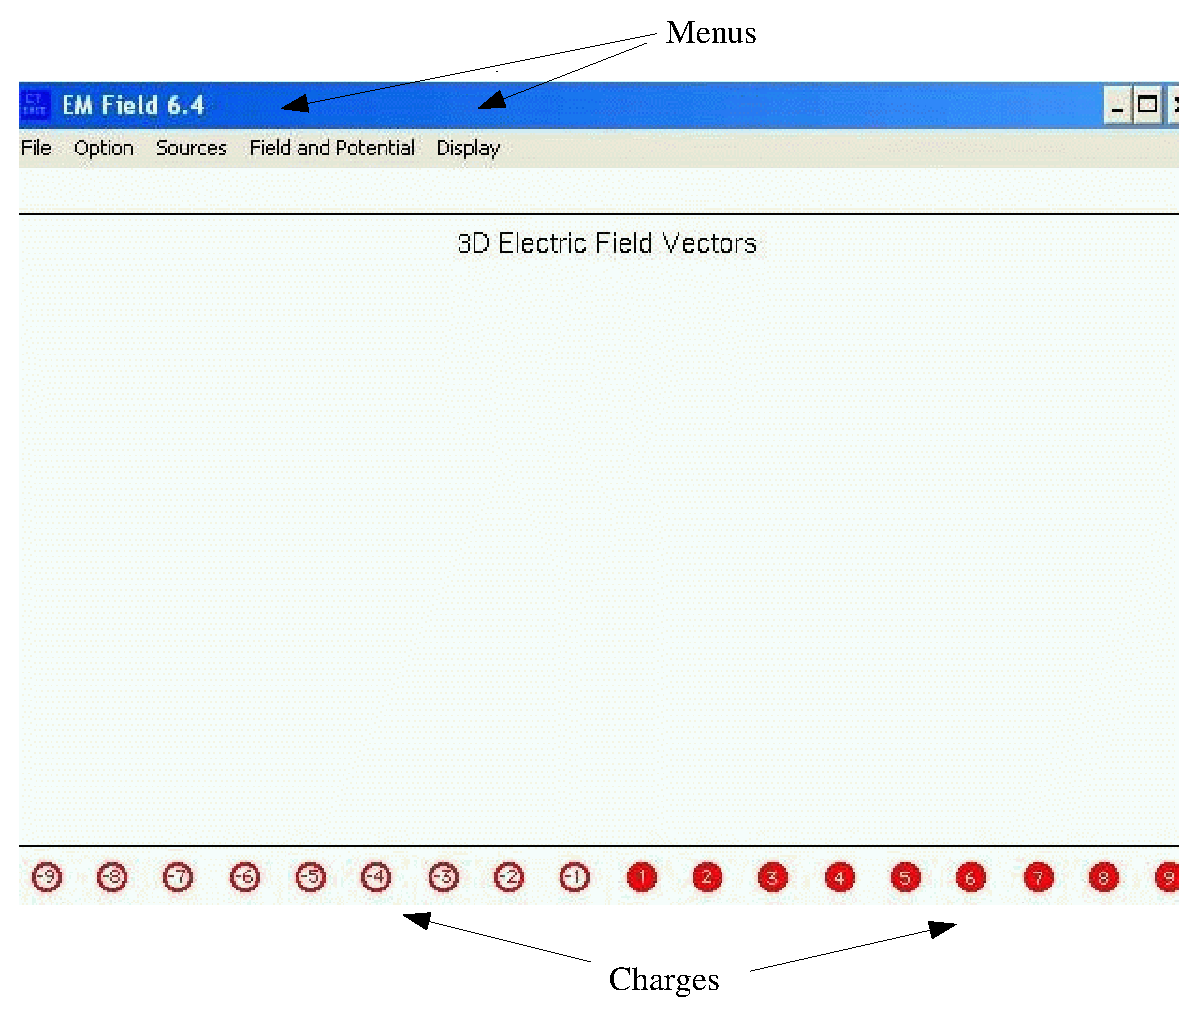
\includegraphics[height=4.0in]{electric_field_and_electric_potential/emfield1c.eps}
\caption{Table top for {\it EMField.}}
\index{color page}
\end{center}
\end{figure}

(b) Go to the {\bf Display} menu and set {\it EMField} to
{\bf Show Grid} and {\bf Constrain to Grid}.
These choices will make the following investigation a bit easier to perform.

(c) Select
the charge labeled {}``+4'' from the available set by clicking
on it and dragging it to the center of the table top. 

(d) \textbf{Prediction}: You will take measurements of the field at different
distances from the charge. You know the relative size of the
charge (+4), but you don't know the size of the charge in coulombs.
Generate an expression for the magnitude of the field from an unknown charge
with appropriate numerical constants and units.
The only unknown in your result should be the charge in coulombs.
How does the electric field depend on $r$, the distance from the point charge?
%\vspace{15mm}
\newpage

(e) Click anywhere in the table top and you will see an arrow drawn.
The size and direction of the arrow represent the magnitude and direction of
the electric field at that point due to the `+4' charge.
In what direction does the arrow point?
Click on the opposite side of the table top.
In what direction does this arrow point? How is it related to the first arrow?
\vspace{15mm}

(f) Click on many points so that you get a wide range of magnitudes from large
(barely fits on the table top) to small (barely bigger than a dot).

(g) Print the table top and use a ruler to measure the distance of each field 
point from the charge and the lengths of each of the arrows on your plot. 
Enter these data in the table below. Use the scale at the bottom of the table 
top to convert the length of each arrow into an electric field magnitude.
The units of the scale electric field vector are $1.0 ~ N/C$.

\vspace{0.3cm}
{\centering \begin{tabular}{|c|c|c|c|}
\hline 
~~~Distance from Charge (cm)~~~&
~~~Arrow Length (cm)~~~&
~~~Measured E (N/C)~~~\\
\hline
\hline 
&
&
\\
\hline 
&
&
\\
\hline 
&
&
\\
\hline 
&
&
\\
\hline 
&
&
\\
\hline 
&
&
\\
\hline 
&
&
\\
\hline 
&
&
\\
\hline 
&
&
\\
\hline
\end{tabular}\par}
\vspace{0.3cm}

%(h) Use the results in column 3 of your table to determine the unknown charge for each electric field measurement and enter the results in the table. NOTE: 
%For this calculation, assume the Coulomb's Law constant $k = 1.00 Nm^{2}/C^{2}$.
%This makes the charge a factor of about $10^{10}$ bigger than it is supposed to 
%be, but we are focussing here on how the electric field varies with distance 
%from the charge. Calculate the average and standard deviation of the values 
%of the charge. Are your results consistent? Explain.
%\vspace{30mm}

(h) \textbf{Prediction}: From Coulomb's Law, we expect the spatial variation
of the field strength to obey a power law: \( \left| E\right| =Ar^{n} \),
where \( A \) and \( n \) are constants. What do you predict the value of 
\( n \) to be?\vspace{15mm}

(i) Graph field strength as a function of $r$. Using the power fitting
function, determine the power of the function, $n$, and record it here.
Attach the plot to this unit.
\vspace{15mm}

(j) Does your result agree with your prediction? Explain any discrepancy.
\vspace{15mm}

\vspace{0.5in}
\textbf{Activity 2: The Electric Potential}

(a) Under the {\bf Display} menu click on {\bf Clean up Screen} to erase the
electric field vectors.

(b) \textbf{Prediction}: You will now take measurements of the potential.
How do you expect the electric potential to change with distance from the point
charge?
\vspace{15mm}
 
(c) Click on the \textbf{Potential} option under the \textbf{Field and Potential} menu. Click on the table top and a marker will be
placed at that point and labeled with the value of the potential there.
Click on many spots on the table top from very close to the point charge to
far away.
When you are finished print the table top.
\vspace{5mm}

(d) Measure and record in the following table the values of the distance from the point charge and the potential.

\vspace{0.3cm}
{\centering \begin{tabular}{|c|c|}
\hline 
~~~Distance (cm)~~~&
~~~Measured V (volts)~~~\\
\hline
\hline 
&
\\
\hline 
&
\\
\hline 
&
\\
\hline 
&
\\
\hline 
&
\\
\hline 
&
\\
\hline 
&
\\
\hline 
&
\\
\hline 
&
\\
\hline
\end{tabular}\par}
\vspace{0.3cm}


%(e) Calculate the value of the electric potential at each of these points
%from the distance you measured from the point charge and the value of the 
%charge from the previous activity. Again, assume $k = 1.00 Nm^{2}/C^{2}$.
%Fill in the appropriate columns of the table  with the distance
%and predicted potential. Show a sample calculation in the space below.
%\vspace{1in}


%(f) Did the measured values agree with your calculations? If they didn't,
%can you explain why not?\vspace{25mm}

(e) \textbf{Prediction}: From Coulomb's Law and the definition of the
electric potential, we expect the spatial variation of the potential
to obey a power law: \( \Delta V=Br^{m} \), where \( B \) and \( m \)
are constants. What do you predict the value of \( m \) to be?
\vspace{12mm}

(f) Graph the voltage as a function of $r$. Using the power fitting
function, determine the power of the function, $m$, and record it here.
\vspace{12mm}

(g) Does your result agree with your prediction? Explain any discrepancy.
\vspace{12mm}

\textbf{Activity 3: Field Lines and Equipotentials}

(a) Under the {\bf Display} menu click on {\bf Clean up Screen} to erase the 
potential values.

(b) Click on {\bf Field Lines} under the {\bf Field and Potential} menu. Click on many spots on the table top all around the charge to create field lines. Why are they straight lines?
\vspace{30mm}

(c) Click on {\bf Directional Arrows} under the {\bf Field and Potential} menu. Click on many spots to create directional arrows for the field lines. (Remember, electric field is a vector quantity.) Why are they directed away from the charge?
\vspace{30mm}

(d) Click on {\bf Equipotentials} under the {\bf Field and Potential} menu. Click on many spots to create equipotential lines. Why are they all circular?
\vspace{30mm}

(e) What is the relationship between the field lines and the equipotentials at 
the points where they cross?
